\chapter{Simulation and Results}
\label{chap4}
In the previous chapter, we have discussed about our methodology for this project while giving details about block diagram, system model, flow chart, software selection of this project. In this chapter, we will provide the viewable logical topology, and results of the project.
\section{Simulation Results}
As discussed in the previous chapter in the section of software selection, we have used Cisco Packet Tracer to simulate our project.
\subsection{Logical Topology}
In the Fig. \ref{mainBranchCampus} a main branch topology is shown which contain three departments, Electrical and Computer Engineering Department, Mathematics Department, Admission Department, and a Cloud Server.
\begin{figure}[H]  %h=positioning
\begin{center}
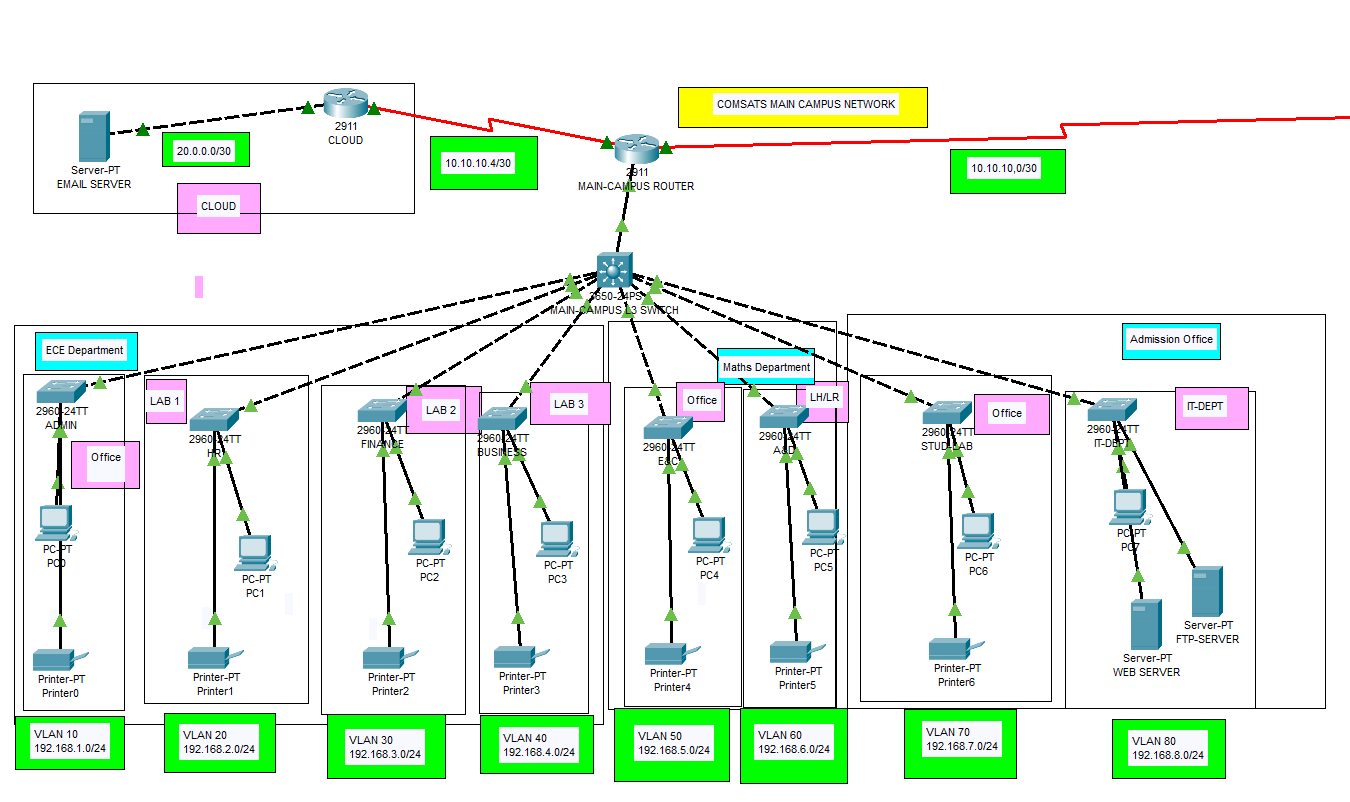
\includegraphics[scale=0.43]{Chapter4/mainBranchCampus}
\caption{Main Branch Topology}
\label{mainBranchCampus}
\end{center}
\end{figure}
Whereas in Fig. \ref{branchCSDepartment}, department of Computer Science is shown which contains different offices and lab. The reason we called this COMSATS Branch Campus is because it is quite apart from the other department in this case we can consider this as a Branch Campus. We can include this in the main branch too but the reason of treating this as a campus is to learn how to connect campus network with the main network.
\begin{figure}[H]  %h=positioning
\begin{center}
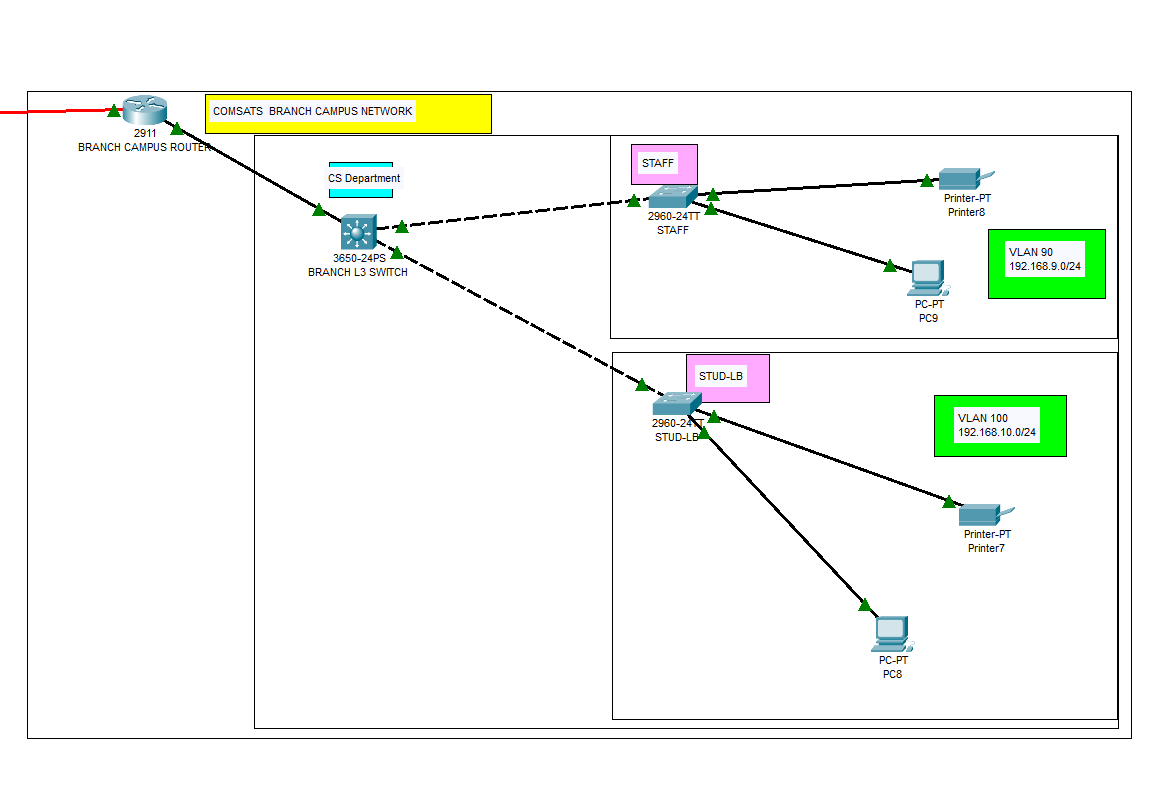
\includegraphics[scale=0.50]{Chapter4/branchCSDepartment}
\caption{Branch Topology of CS Department}
\label{branchCSDepartment}
\end{center}
\end{figure}
\subsection{Statistical Analysis}
\label{analysis}
Fig. \ref{resultSimulation} shows the results of the simulation. In which, we have forwarded a message from source host i.e., PC0 to the destination host i.e., PC4.\\
\begin{figure}[H]  %h=positioning
\begin{center}
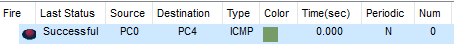
\includegraphics[scale=1.3]{Chapter4/resultSimulation}
\caption{Simulation Results}
\label{resultSimulation}
\end{center}
\end{figure}
Fig. \ref{simulationPanel} it's showing a complete path which it follows to reach to the destination host and than acknowledge back to the source host with the time it take while using Internet Control Message Protocol (ICMP) which is a network layer protocol used by network devices to communicate.
\begin{figure}[H]  %h=positioning
\begin{center}
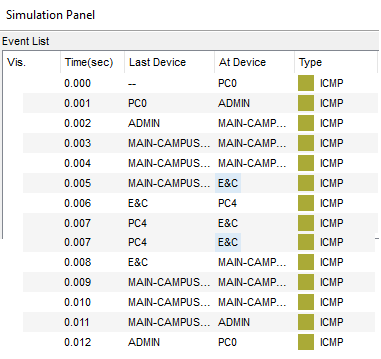
\includegraphics[scale=1.0]{Chapter4/simulationPanel}
\caption{Simulation Panel Results}
\label{simulationPanel}
\end{center}
\end{figure}
\subsection{Using Command Prompt}
\noindent The ping command is a very common method for troubleshooting the accessibility of devices. It uses a series of Internet Control Message Protocol (ICMP) Echo messages to determine:\\
\begin{itemize}
\item Whether a remote host is active or inactive.

\item The round-trip delay in communicating with the host.

\item Packet loss.
\end{itemize}

\noindent The ping command first sends an echo request packet to an address, then waits for a reply. The ping is successful only if:
\begin{itemize}
\item the echo request gets to the destination, and

\item the destination is able to get an echo reply back to the source within a predetermined time called a timeout. The default value of this timeout is two seconds on Cisco routers.
\end{itemize}
\noindent Fig. \ref{commandPrompt} shows a different way to check if our network connectivity is reliable. We have used command prompt of PC2 and have ping two hosts: one from the branch/CS Department host i.e, PC8 with IP address 192.168.10.2/24 and second from Admission Department host's i.e., PC6 with IP address 192.168.7.2/24.
\begin{figure}[H]  %h=positioning
\begin{center}
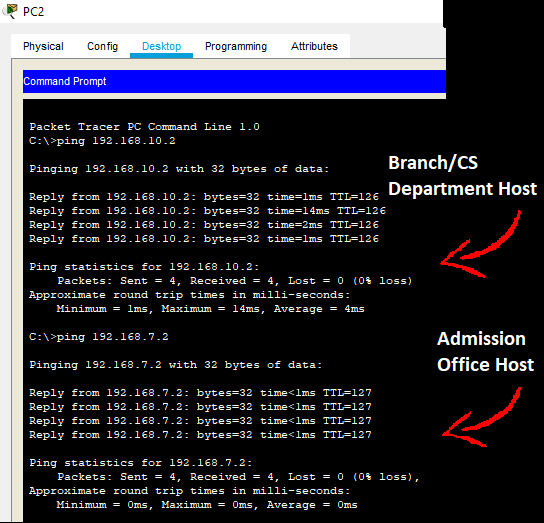
\includegraphics[scale=1.0]{Chapter4/commandPrompt}
\caption{Command Prompt Results}
\label{commandPrompt}
\end{center}
\end{figure}



